\section{Manual de usuario}\label{sec:manual_usuario}
El usuario final, es decir, alguna de las partes interesadas
(ver~\ref{sec:stakeholders}), interacciona con el sistema a través del
servicio de Kibana, accesible a través de cualquier navegador web a través
del subdominio DNS definido en la configuración de Terraform.

Puesto que el servicio está disponible en la red pública, es necesario
autenticarse para poder acceder a él. Para ello, se debe introducir el
usuario y contraseña generados durante el despliegue de la infraestructura.

\begin{figure}[H]
	\centering
  	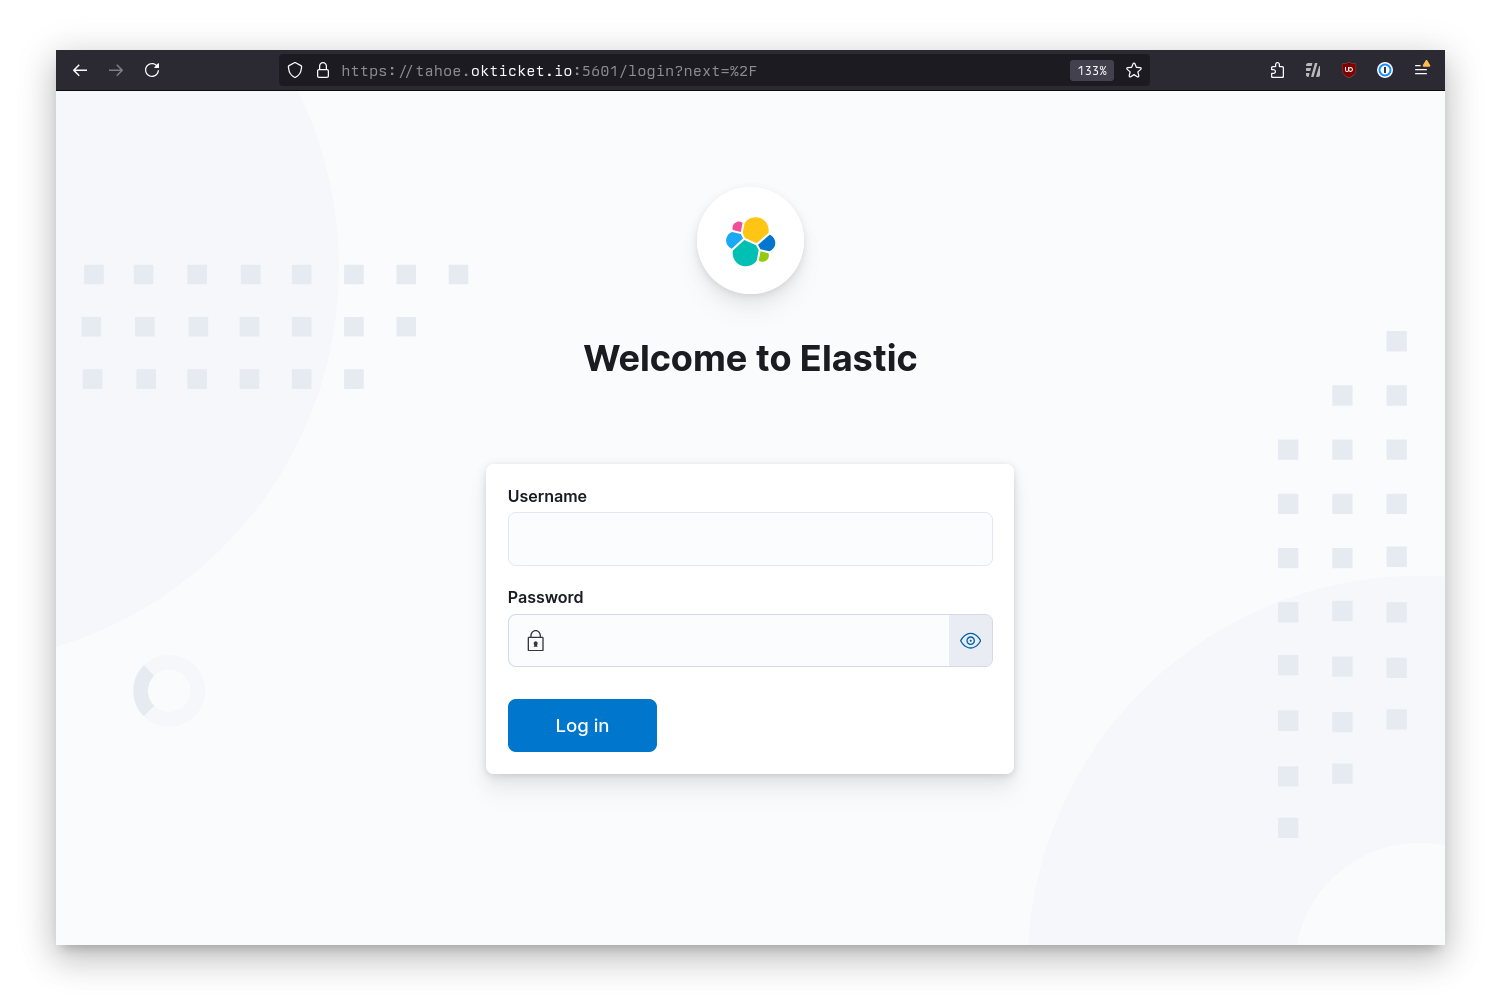
\includegraphics[width=\textwidth]{manual/kibana_login.png}
  	\caption{Pantalla de inicio de sesión de Kibana}
  \label{fig:login}
\end{figure}

\emph{NOTA: se utilizan datos y paneles de ejemplo para ilustrar el manual.}

\subsection{Usuario normal}
Una vez introducidos los datos de acceso, Kibana redirige el usuario a la
página por defecto configurada para su rol, que para el usuario final debería
ser siempre el listado de \textit{dashboards}.

\begin{figure}[H]
	\centering
  	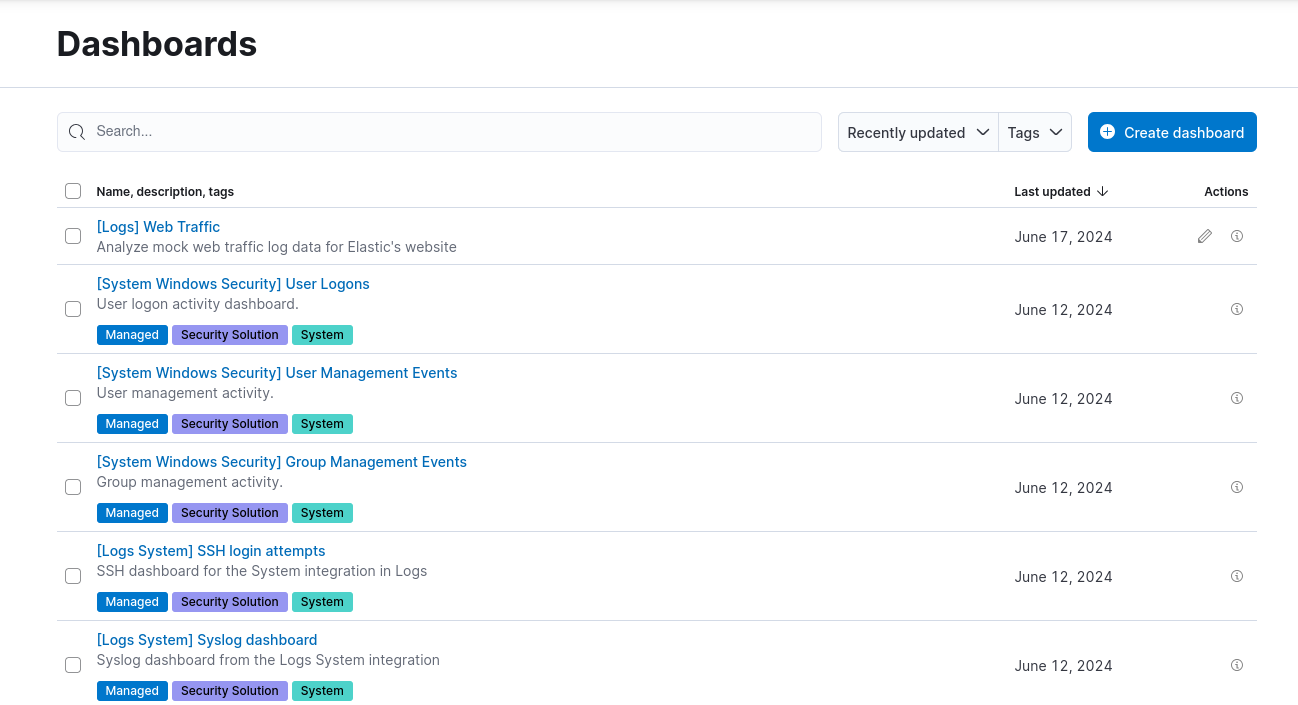
\includegraphics[width=\textwidth]{manual/dashboards.png}
  	\caption{Listado de dashboards de Kibana}
  \label{fig:dashboards}
\end{figure}

Dentro de la lista de \textit{dashboards}, el usuario puede seleccionar
cualquiera a los que tenga acceso para visualizar los datos en tiempo real.
En el caso del equipo de desarrollo, tendrán acceso a todos los paneles y
podrán modificar y crear nuevos.

\begin{figure}[H]
	\centering
  	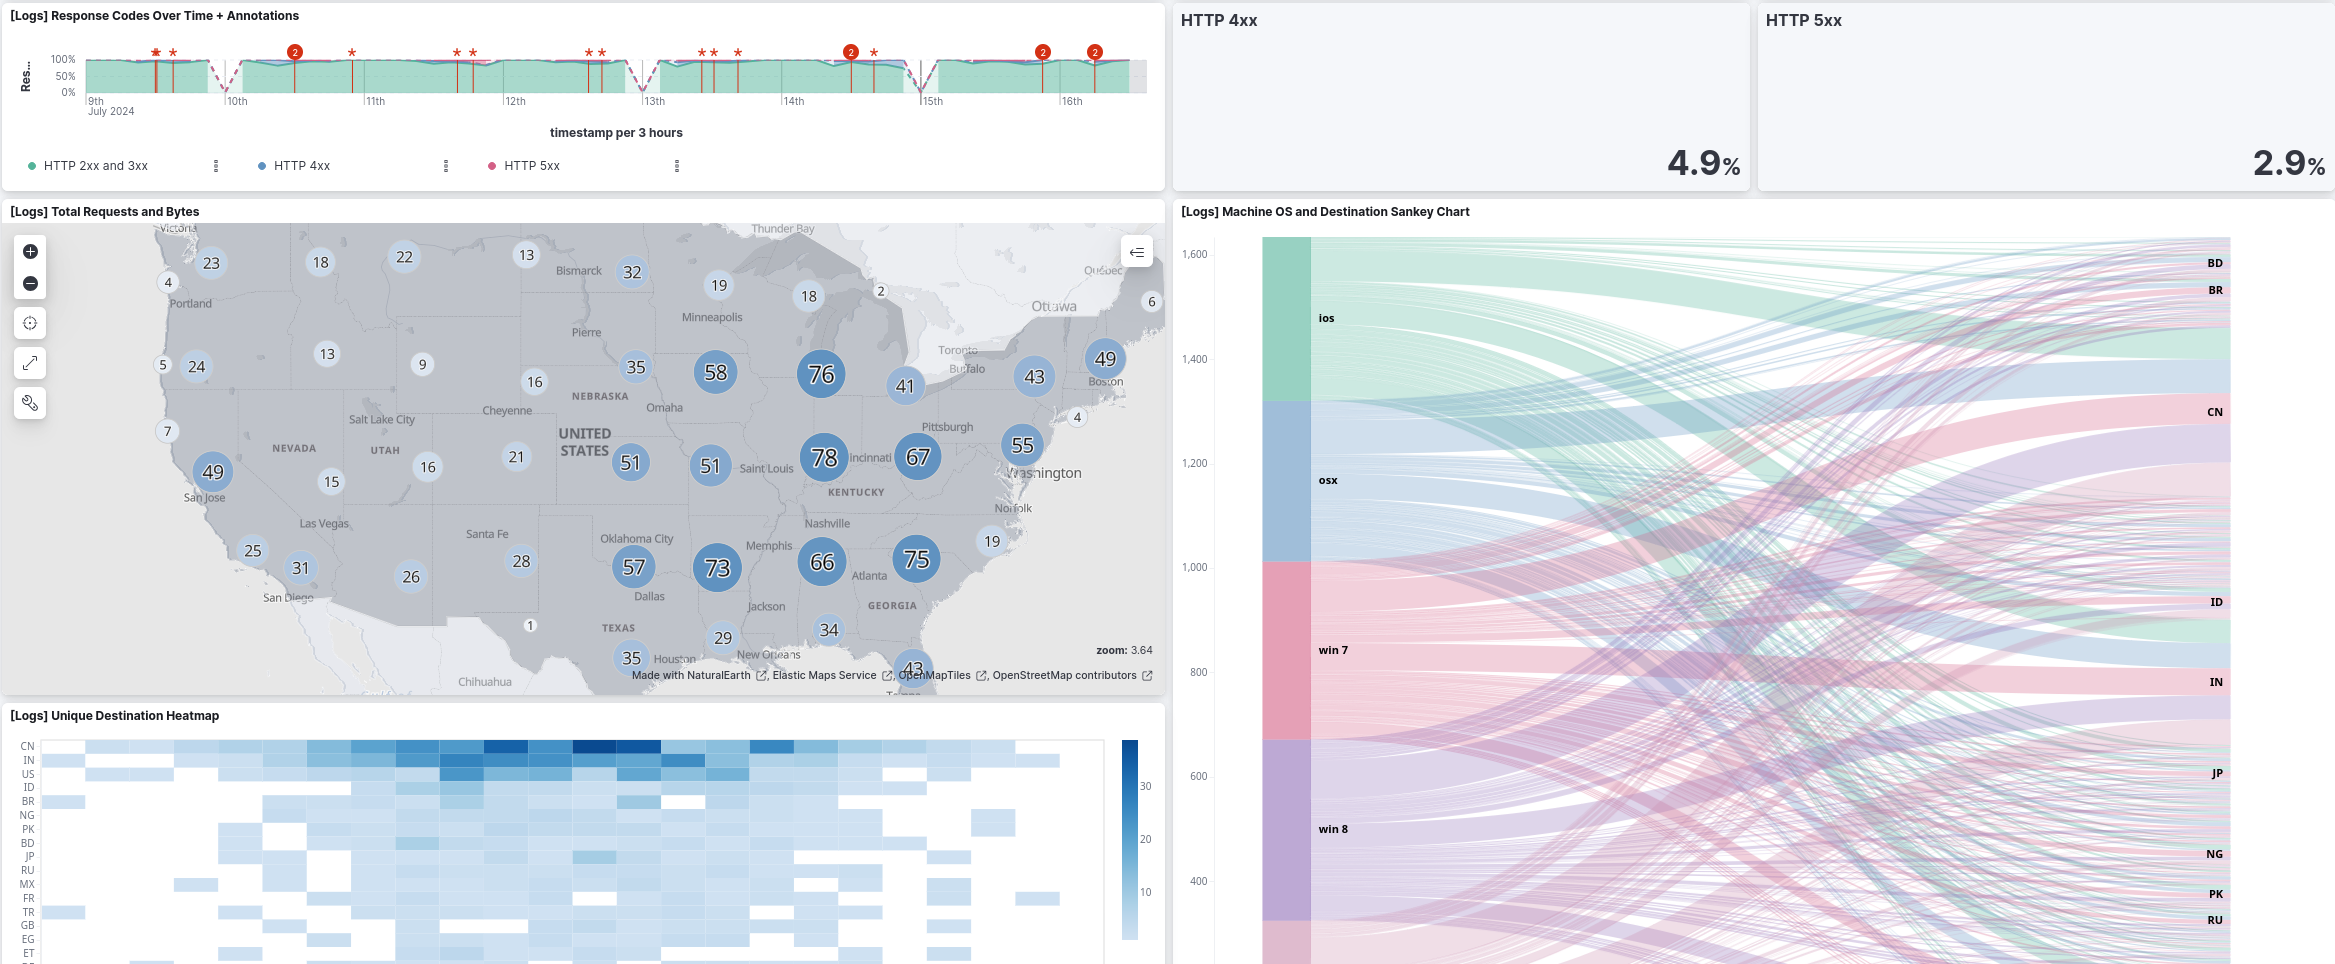
\includegraphics[width=\textwidth]{manual/dashboard.png}
  	\caption{Ejemplo de dashboard de Kibana}
  \label{fig:dashboard}
\end{figure}

En la parte superior de la pantalla, el usuario puede seleccionar el rango de
tiempo que desea visualizar, así como el intervalo de actualización de los
datos. Además, puede seleccionar el rango de tiempo de forma manual.

También existe la posibilidad de filtrar la información mostrada en el panel
según diferentes campos, bien haciendo uso de los filtros predefinidos o
haciendo consultas personalizadas en el campo de búsqueda con sintaxis KQL
\footnote{\url{https://www.elastic.co/guide/en/kibana/current/kuery-query.html}}.


\subsection{Usuario administrador}
Aquellos usuarios con permisos de administración podrán además acceder a otras
partes más avanzadas de Kibana, como la monitorización y creación de alertas o
la gestión de usuarios y roles.

\begin{figure}[H]
	\centering
  	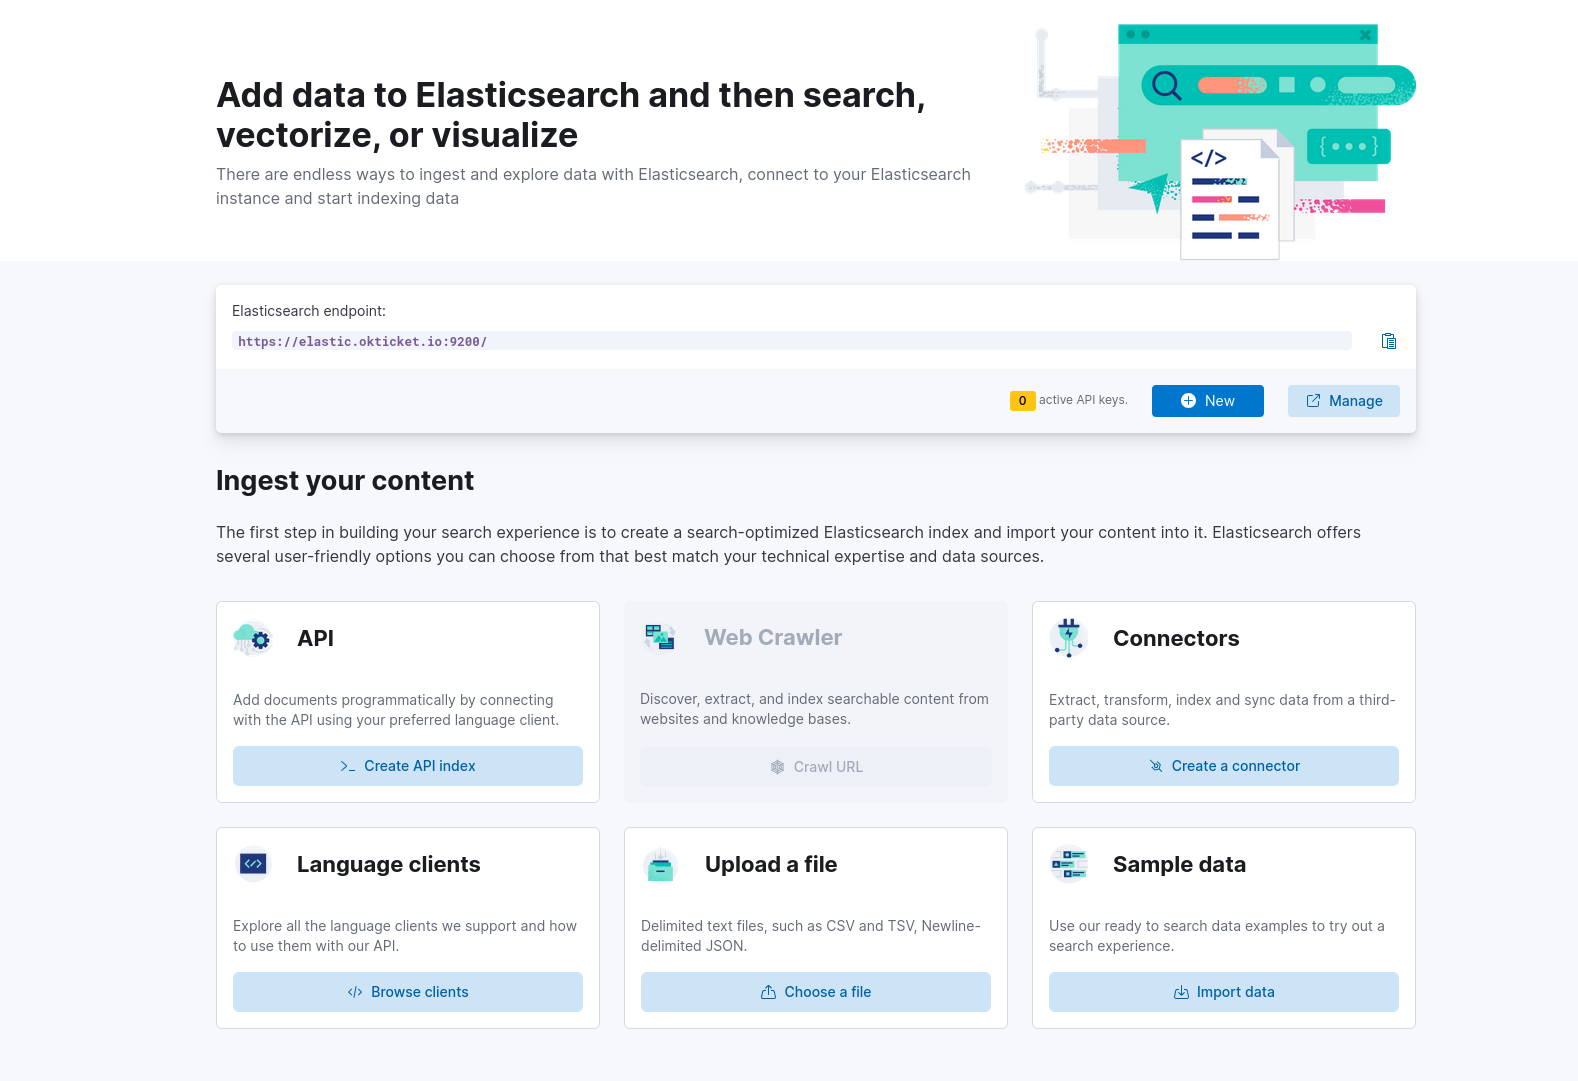
\includegraphics[width=\textwidth]{manual/kibana_config.png}
  	\caption{Opciones de fuentes de datos de Elasticsearch a través de Kibana}
  \label{fig:kibana_config}
\end{figure}

\begin{figure}[H]
	\centering
  	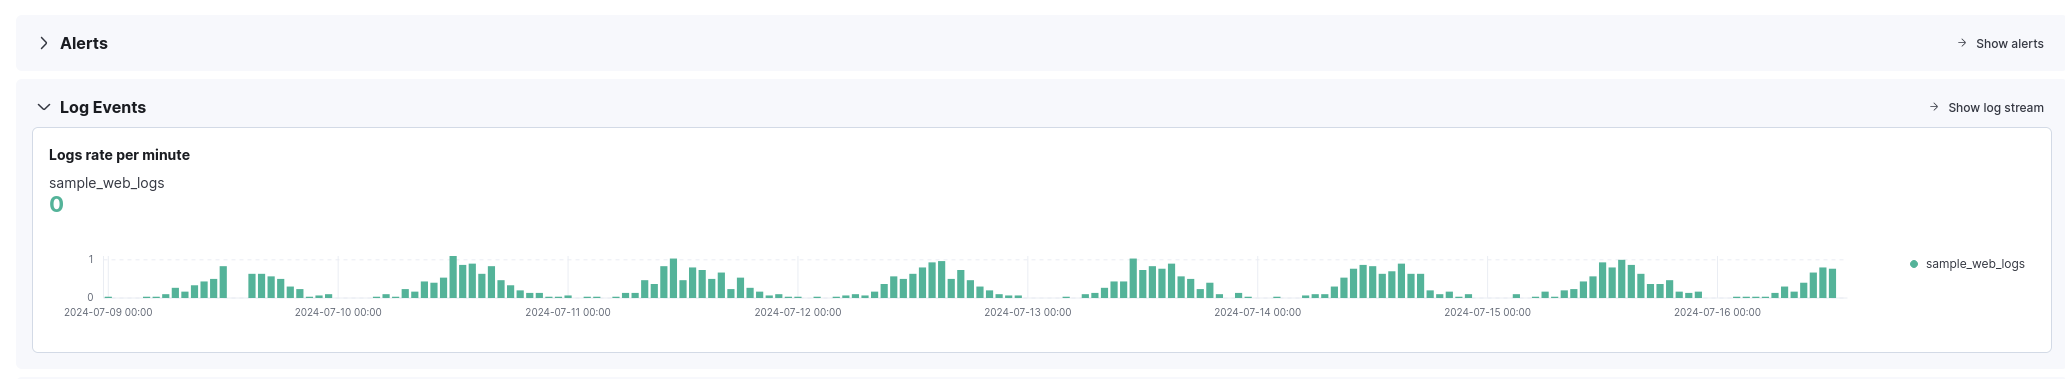
\includegraphics[width=\textwidth]{manual/kibana_alerts.png}
  	\caption{Ejemplo de alertas y métricas en Kibana}
  	\label{fig:kibana_alerts}
\end{figure}
